Pneumatic mechanism is also a potential solution.
Its main advantage is that the power source is divorced from the actuator \cite{russomanno_design_2015}.
Power, in the form of pressurized air, is routed via small pipes and readily converted into the motion of a sliding pin using an elastic membrane.
This feature of separation of power source and functional module make pneumatic design promising in terms of forming a large-area dense array shape display.
However, one big challenge of pneumatic design is how to efficiently control large number of cells without sacrifice of portability \cite{russomanno_model-based_2017}.
The group proposed a fluidic logic system design shown in figure \ref{fig:pneumatic-schema} to solve this problem and the prototype showed positive results in the earlier tests \cite{russomanno_design_2015}.

\todo[inline]{``managed to release'' and ``still in pre-order''. I'd argue this needs to be more dismissive of their product and its promises as part of the reason why we wont want to touch fluids.}
Blitab annouced the start of pre-order of their pneumatic-based product in 2017, as shown in Fig.7 However, the official product release was delays and until now the product has not reached the market for unknown reasons. The product was claimed to be sold at 500 USD and looks very promising in their official videos. However, the complexity of the necessary fluidic logic system and budgetary constraints of the project combined with the possible complications they must have encountered to have to delay the release of the product, make this design unsuitable for the scopes of this project.

\begin{figure}\centering
    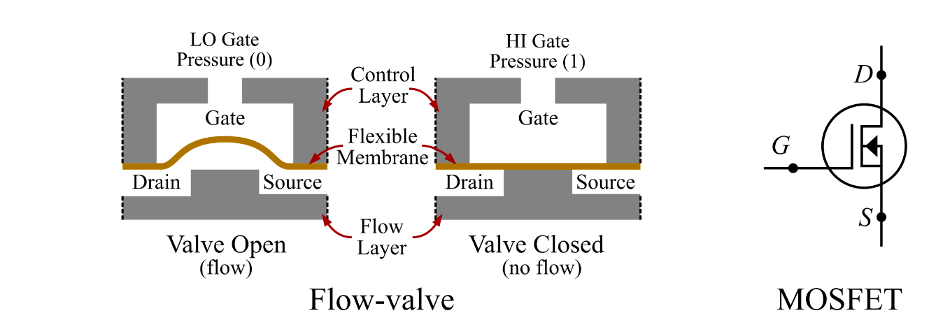
\includegraphics[width=0.6\textwidth]{figures/pneumatic-schema.png}
\caption{Cross-sectional views of a pressure-based fluidic valve in the open and closed states.}
\label{fig:pneumatic-schema}
\end{figure}

\begin{figure}\centering
    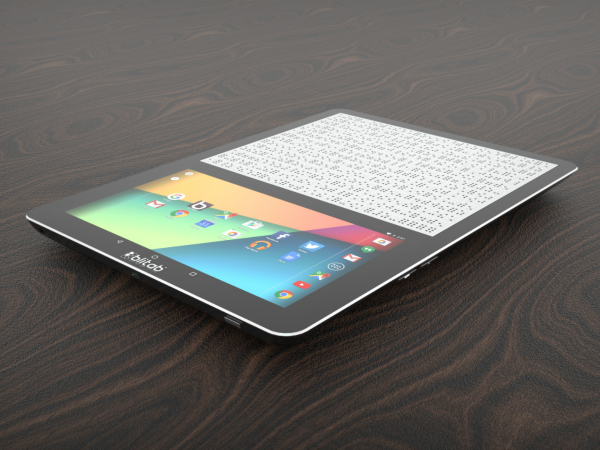
\includegraphics[width=0.6\textwidth]{figures/Blitab_product.jpg}
\caption{Blitab's Pneumatic-based braille display}
\label{fig:Blitab-product}
\end{figure}